\chapter{Case}
\section{Background}
There has been some interest in the area of \gls{sms} reporting from the \gls{uio}.
The \gls{dhis2} software supporting this functionality has been developed, but not yet been used.
The \gls{hmis} team at the \gls{moh} in Rwanda has for some time been wanting to use \gls{dhis2} in order to make a system for keeping track of \gls{chw}'s essential drugs and supplies. The system, \gls{clmis}, should be able to track \gls{chw}'s stock and distributions of these items. 
The \gls{hmis} team are actually working for the \gls{chd} who are the clients in this case. 
The current system is primarily a pull system where \gls{chw}'s make monthly visits to their local \gls{hc} \gls{chw} supervisors in order to resupply. 
\begin{quotation}
In order for these \gls{chw}'s to provide uninterrupted care to their communities, it is essential to have access to the essential drugs and supplies these health workers dispense.
\end{quotation}

Rwanda is now in the process of rolling out a national \gls{elmis} that is supposed to cover all levels of the health system, but this does not include the $\approx 45000$\gls{chw}'s in $\approx 15000$villages.
This is were the \gls{clmis} comes in. 
With \gls{dhis2} as a base software \gls{chw}'s will be able to report data on what they receive and has in stock of the essential drugs and supplies. 
Further, the plan is to integrate \gls{clmis} with the national \gls{elmis} in order to have interoperability between systems. 

\section{Networks of Action}
As mentioned by Eric, Jørn and Sundeep, one key to make this possible is the network of action. 
As a student-researcher I've been able to get a position as an intern at \gls{msh}.  
The core of this initiative is the \gls{chd}. They have asked \gls{hmis} for support on developing \gls{clmis}. 
The \gls{hmis} team has support from both \gls{msh} and \gls{hisp}. 
\subsection{Description of the different participants here}

\section{Objectives}
\label{sec:objectives}
In order to make the case managable for a research project it was limited to four objectives. 

\begin{description}
\item[\#1:] Send SMS and email notifications based on rules.\label{desc:objectiveone}
\item[\#2:] Send SMS and email reminder if a report is more than 4 days delayed.\label{desc:objectivetwo}
\item[\#3:] If user data does not map correctly user feedback should be provided.\label{desc:objectivethree}
\item[\#4:] A functional SMS based reporting system.\label{desc:objectivefour}
\end{description}

These objectives are somewhat simplified in order to be easier to work with. A more elaborate description folllows. 
\subsection{Objective \#1}
Notifications here are meant as in the broadest of meanings. The idea is that the system should be able to communicate with the \gls{chw}'s based on some configuration. In this case, a notification could mean a resupply order or an alert. Rules would then be related to thresholds or algorithms. For an example, resupply order would be generated by an algorithm that calculates how much of each supply item the \gls{chw} needs. 
\subsection{Objective \#2}
This objective is straight forward. If a \gls{chw} in charge of reporting at a village does not report after 4 days of the previous reporting month, a reminder should be sent. 
\subsection{Objective \#3}
Sometimes when a \gls{chw} reports data, syntax error may happen. It is also preferable to have some kind of feedback when everything is just fine. Just to know that everything is working. 
The appropriate instructions for fixing mistakes should also be in the feedback from the system.
\subsection{Objective \#4}
In this case a functional reporting system would be a system that is ready to receive \gls{sms} reports from the \gls{chw}'s. These messages are stored in the \gls{clmis} database ready to be analyzed. 

\section{Refining and Defining the Requirements}
As a part of a diagnosis we started out with trying to define usecases for each of the objectives. 
This would make it more clear what needed to be done in order to meet them.
It was very diffiult to pinpoint exactly what needed to be done bacause of the projects size. 
\gls{hmis} was in charge of configuring and develop the system. \gls{hmis} was doing this for the \gls{chd}, both located in the the same department, \gls{moh}. 
Collecting the requirements would then be based on what we understood from what the \gls{chd} could tell us. \gls{hmis} had already made some progress on this part.  

\begin{figure}
\centering
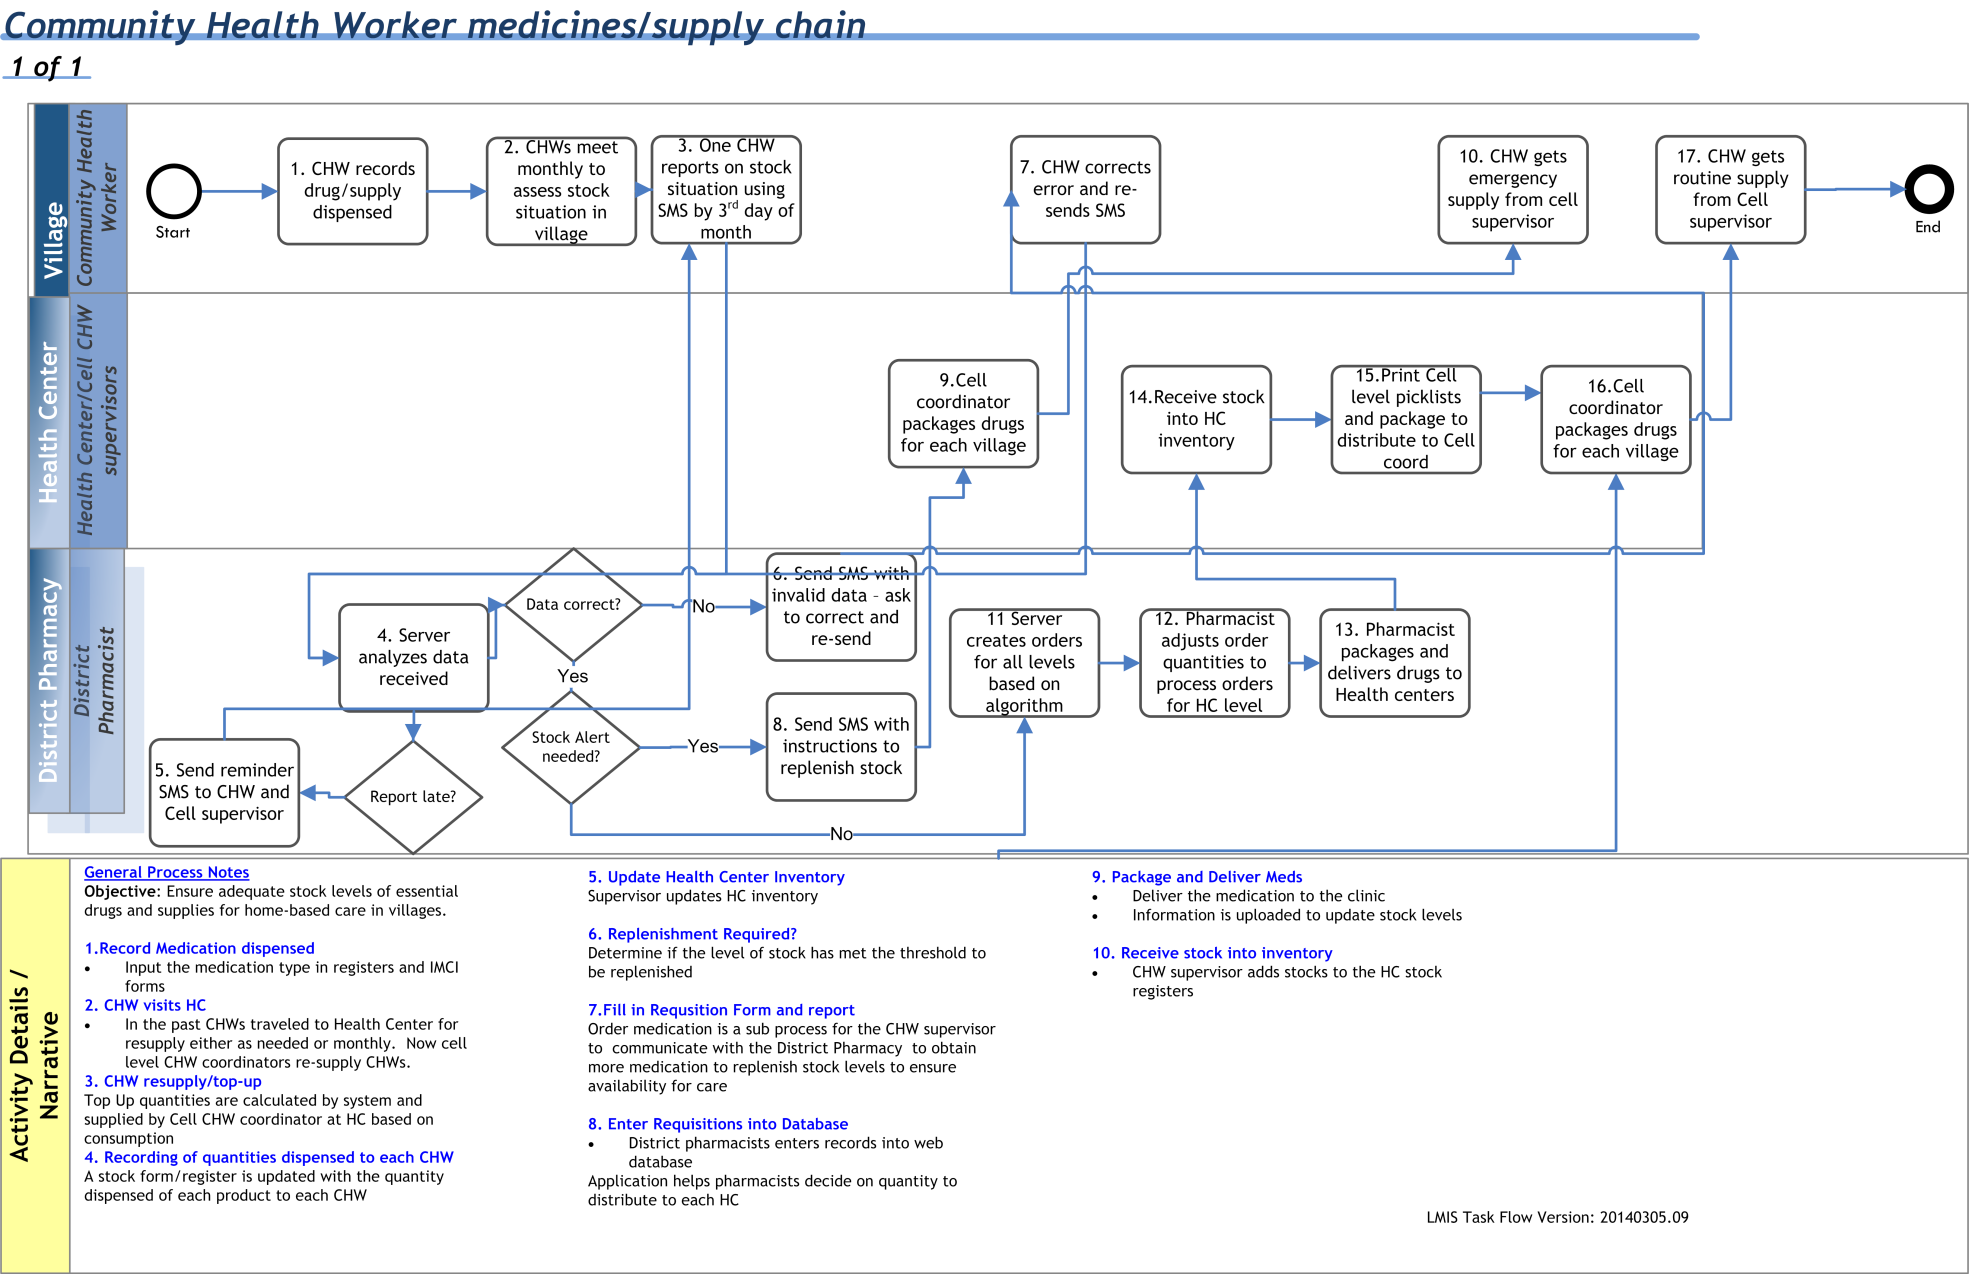
\includegraphics[width=\textwidth]{case/img/chwSupplyChainFuture}
\caption{\gls{chw} Supply Chain in the Future}
\label{fig:chwSupplyChainFuture}
\end{figure}

Figure \ref{fig:chwSupplyChainFuture} shows the desired \gls{bpm}. The specifics did not allways match what had previously been discussed, but the important part was to get an overall picture of how thing should work. For an example we will see that the \gls{chw}'s would rather report on what they receive instead of what they dispense. After analyzing the \gls{chw} supply chain \gls{bpm} we found the following. 
Activity 1, 2, 3, 7 was supported as long as the \gls{chw} had a mobile phone. After discussing it with one of \gls{chd}'s team members, it was fairly safe to assume this. 
Activity 4 relates directly to objective \#4.
Activity 6 relates to objective \#3. 
Activity 5 relates to objective \#2 and Activity 8 and 11 to objective \#1. Activity 9--10, 12--17 should supported as long as the objectives were met. 
This puts our objectives in context of a bigger picture.

\subsection{Use Cases}
\begin{table}
	\centering
	\begin{tabular}{|p{5cm}|p{7cm}|}
		\hline
		\multicolumn{2}{|c|}{\textbf{Send SMS and Email Notifications}}\\
		\hline
		\textbf{Goal:} & Create orders\\
		\hline
		\textbf{Primary Actor:} & System\\
		\hline
		\multirow{3}{*}{\textbf{Secondary Actor:}}	& Cell CHW Supervisor \\
																								& HC CHW Supervisor \\ 
																								& District Pharmacist \\
		\hline
		\multirow{4}{*}{\textbf{Main Success Scenario:}}	& 1. CHW reports distributed and stock values. \\
																											& 2. System processes report. \\
																											& 3. System calculates essential drugs needed for each level. \\
																											& 4. System sends orders to cell, sector and district. \\
		\hline
		\textbf{Extensions:} & \\
		\hline
	\end{tabular}
	\caption{Textual Use Case: Send SMS and Email Notifications}
	\label{tab:notifications}
\end{table}


\begin{table}
	\centering
	\begin{tabular}{|p{5cm}|p{7cm}|}
		\hline
		\multicolumn{2}{|c|}{\textbf{Send SMS and Email Reminders}}\\
		\hline
		\textbf{Goal:} & Send reminder \\
		\hline
		\textbf{Primary Actor:} & System \\
		\hline
		\multirow{2}{*}{\textbf{Secondary Actor:}}	& CHW \\
																								& Cell CHW Supervisor \\
		\hline
		\multirow{5}{*}{\textbf{Main Success Scenario:}}	& 1. CHW misses report deadline. \\
																											& 2. 5 days goes by. \\
																											& 3. System sends reminder by email and SMS. \\
																											& 4. Another 5 days goes by. \\
																											& 5. System sends reminder by email and SMS. \\
																											
		\hline
		\textbf{Extensions:} & \\
		\hline
	\end{tabular}
	\caption{Textual Use Case: Send SMS and Email Reminders}
	\label{tab:reminders}
\end{table}


\begin{table}
	\centering
	\begin{tabular}{|p{5cm}|p{7cm}|}
		\hline
		\multicolumn{2}{|c|}{\textbf{Send Report Feedback}} \\
		\hline
		\textbf{Goal:} & Process SMS message\\
		\hline
		\textbf{Primary Actor:} & System \\
		\hline
		\textbf{Secondary Actor:} & Community Health Worker \\
		\hline
		\multirow{6}{*}{\textbf{Main Success Scenario:}}	& 1. CHW reports data incorrectly by SMS. \\
																											& 2. System receives SMS. \\
																											& 3. SMS triggers feedback message. \\
																											& 4. CHW corrects message and re-sends report. \\
																											& 5. System processes SMS. \\
																											& 6. System updates database. \\
		\hline
		\textbf{Extensions:} & \\
		\hline
	\end{tabular}
	\caption{Textual Use Case: Send Report Feedback}
	\label{tab:feedback}
\end{table}

\begin{table}
	\centering
	\begin{tabular}{|p{5cm}|p{7cm}|}
		\hline
		\multicolumn{2}{|c|}{\textbf{Report Using SMS}}\\
		\hline
		\textbf{Goal:} & Update Database \\
		\hline
		\textbf{Primary Actor:} & Community Health Worker\\
		\hline
		\textbf{Secondary Actor:} & System \\
		\hline
		\multirow{5}{*}{\textbf{Main Success Scenario:}}	& 1. CHW reports stock and distributed values of essential drugs. \\
																											& 2. System receives SMS. \\
																											& 3. System processes SMS. \\
																											& 4. System updates database. \\
																											& 5. System sends confirmation SMS to CHW. \\
		\hline
		\textbf{Extensions:} & \\
		\hline
	\end{tabular}
	\caption{Textual Use Case: Report Using SMS}
	\label{tab:smsreport}
\end{table}

As a seen in use case tables \ref{tab:notifications}, \ref{tab:reminders}, \ref{tab:feedback} and \ref{tab:smsreport}, the specifics did change, along with the development process, but it gave us the necessary guidelines to understand the desired outcome.
The obstacles then became somewhat clearer. The \gls{chw}'s needed a server to communicate with and the server needed to be able to communicate with the \gls{chw} supervisors at the different levels in the health hierarchy.
The communication channels that should be used between the system and the users would be email and \gls{sms}. Email support are possible to set-up without involving any other parties, but \gls{sms} on the other hand are somewhat tricker. Here we have to include a mobile company in order to proparly test the service. This service also includes using software and hardware outside of the department.


\section{Planning}
\begin{figure}
\centering
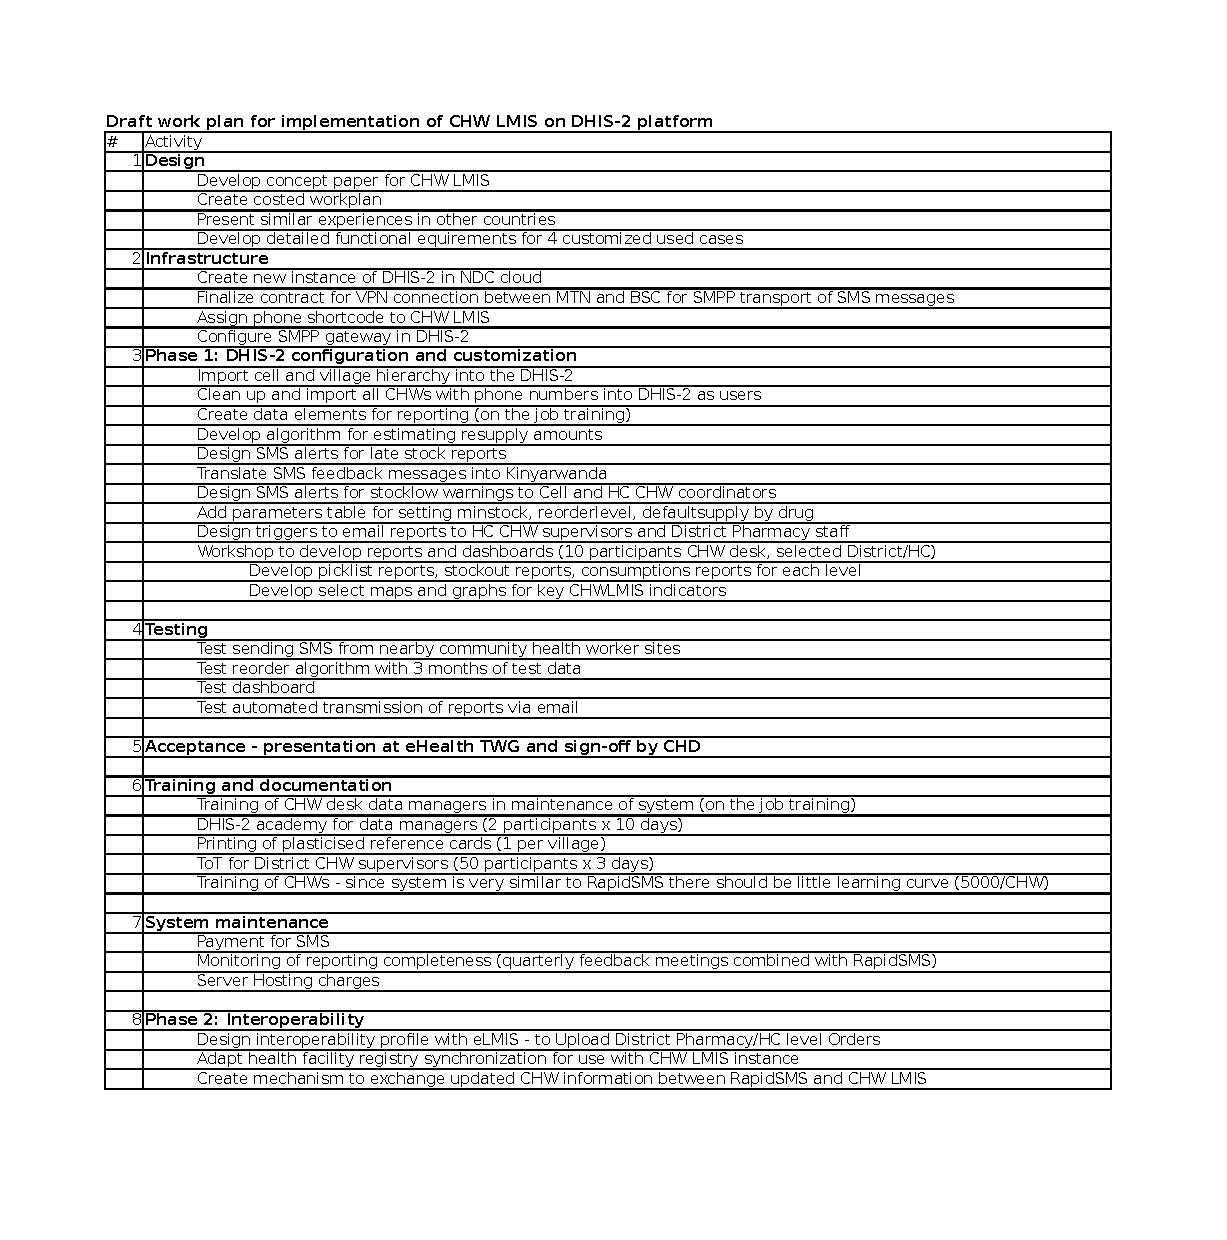
\includegraphics[width=\textwidth]{case/img/lmisWorkPlan}
\caption{Activity Plan For the \gls{chw} \gls{lmis}}
\label{fig:activityPlan}
\end{figure}
With the objectives put in context we could start planning the specific activites for intervention. 
In our case the \gls{hmis} team made the overall plan for the project as in figure \ref{fig:activityPlan}.
The objectives then relates to the following points of intervention, take into account that there are dependencies along the different activities. 
\begin{description}
\item[\textbf{Objective \#1}]\hfill
	\begin{description}
	\item[3.4]Develop algorithm for estimating resupply amounts.
	\item[3.7]Design SMS alerts for stocklow warnings to Cell and HC CHW coordinators.
	\item[3.8]Add parameters table for setting minstock, reorderlevel, defaultsupply by drug.
	\item[3.9]Design triggers to email reports to HC CHW supervisors and District Pharmacy staff.
	\end{description}
\item[\textbf{Objective \#2}]\hfill
	\begin{description}
	\item[3.5]Design SMS alerts for late stock reports.
	\end{description}
\item[\textbf{Objective \#3}]\hfill
	\begin{description}
	\item[3.6]Translate SMS feedback messages into Kinyarwanda.
	\end{description}
\item[\textbf{Objective \#4}]\hfill 
	\begin{description}
	\item[3.1]Import cell and village hierarchy into the DHIS-2.
	\item[3.2]Clean up and import all CHWs with phone numbers into DHIS-2 as users.
	\item[3.3]Create data elements for reporting (on the job training).
	\end{description}

\end{description}

The \gls{clmis} will in its final state run on servers at the \gls{ndc}.
This would then involve another party when trying to configure and develop the \gls{clmis}. 
Often taken for granted is stable power supply and internet access. 
In our case, this was not the case. On could experience power cuts on a daily basis.
And working directly on a server under these curcumstances is not very productive. 
Taking this into account we decided to set up a test environment that we could work with. 
Making our configurations and testing possible instantly before we make the changes on the live server at the \gls{ndc}. 
This duplicated our work some, but makes it easier to develop and configure. For an example, one does not need to stop everybody's work if one happens to play with the database to much. Also it makes it easier to divide tasks so that they can run in parallell. 

\section{Intervention}
The first thing that needed to be done was to set up the test environment. 


\subsection{Setting up the Test Environment}
The test environment was set up using an Android smart phone and a laptop. 

\begin{figure}
\centering
\caption{Figure of \gls{sms}-flow}
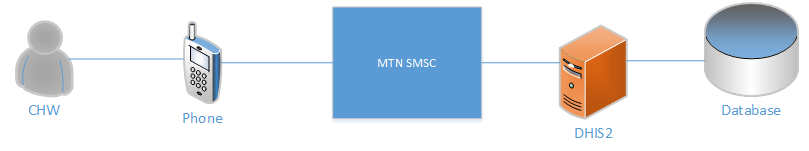
\includegraphics[width=\textwidth]{case/img/smsFlow}
\label{fig:smsFlow} 
\end{figure} 

\begin{figure}
\centering
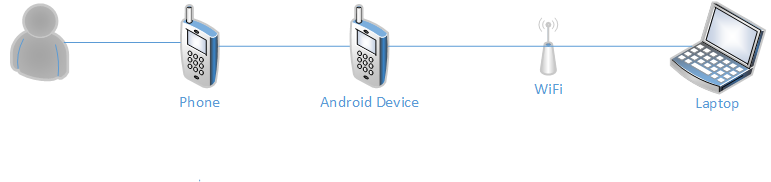
\includegraphics[width=\textwidth]{case/img/testEnvironment}
\caption{Figure of Test Environment}
\label{fig:testEnvironment} 
\end{figure}

Based on advice from the \gls{hisp}-team at the \gls{uio} we chose to use \gls{smpp} protocol in order to transfer \gls{sms}'s from the \gls{chw}'s. In our case, this requires a connection with a \gls{smsc} at a local mobile operator. Typically the \gls{sms} is typed in by the \gls{chw} and sent to a telephone number, usually a four digit number. The message is then received at the \gls{smsc} where it is forwarded to the server at the receiving end for processing. This is an over simplification, but gets the basic idea across. After processing the server is able to send \gls{sms} feedback to the user. In order for us to simulate this at the office space, we chose to use a \gls{sms} gateway application running on a Android device. When a \gls{sms} with the right code word is received, it forwards the \gls{sms} to the server. 

\subsection{Configuring DHIS2}
In order to process the reports \gls{dhis2} has to be ready to receive them.
This involves creating user accounts with the phone number of the sender, creating data elements and sets that make meaning to the values reported and making the codes for the different supplies and drugs that the \gls{chw} reports on. 

\begin{table}
\centering
\begin{tabular}{l l}

\textbf{Data Element Category Combination} &	\textbf{Code} \\
\hline
\textbf{Command} & \textit{stk} \\
amoxicillin\_stk\_eom &	am\\
condom\_stk\_eom & cm\\
injectables\_stk\_eom &	dp\\
mebandazole\_stk\_eom &	mb\\
misoprostol\_stk\_eom &	ms\\
ocp\_stk\_eom &	pp\\
ors\_stk\_eom &	sr\\
primo\_red\_stk\_eom &	pr\\
primo\_yellow\_stk\_eom & py\\
rdt\_stk\_eom &	rd\\
sureau\_stk\_eom & se\\
zinc\_stk\_eom & zn \\
\hline
\end{tabular}
\caption{Codes for Drugs and Supplies}
\label{tab:codesDS}
\end{table}

\begin{figure}
\centering
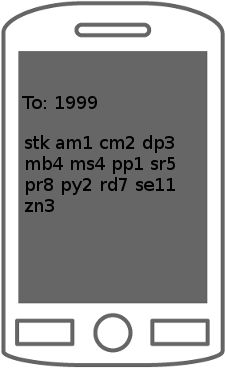
\includegraphics[height=5cm]{case/img/smsExample}
\caption{Example \gls{sms} report}
\label{fig:exsms}
\end{figure}

Table \ref{tab:codesDS} shows names and codes for the drugs and supplies in our case. 
This is data elements for stock at the end of month.
A typical scenario would be that a \gls{chw} counts each item they have at the village the end of the month. Then creates a text message that is sent to the four digit number provided by the mobile operator. Example message in figure \ref{fig:exsms}. In the example message, \textit{stk} is the code word that tells \gls{dhis2} what kind of data is being reported. The first two letters in the message the maps to the different drugs and supplies in the database with the following value.  

\subsection{Demo 1}
After the basic set up we had a short demo for a few members of the \gls{hmis} team. 
This demo showed the most the basic functionality and how we may configure it to fit our requirements. We discussed naming of the different codes and typical issues. One thing was misspelling and user feedback. 
One thing worth taking note of is that a common spelling error was to type the number '1' instead of the letter 'l' and the number '0' instead of the letter 'o'. We solved this by avoiding the letters in the \gls{sms}. Also, we also took note of that many of the users might not be fluid in or even speak English. The local language is 'Kinyarwanda'. An old Buntu language that is very much used even though Rwanda is transitioning to English. \gls{dhis2} is currently not supporting 'Kinyarwanda'.

\subsection{Demo 2}

\subsection{Setting up the mobile instance}
In parallel with the setting up the test environment we began configuring the \gls{dhis2} in the cloud service provided by \gls{ndc}. 
We soon realized that setting up a test environment was worth the time. 
The \gls{ndc} is being administrated and operated by another team outside the \gls{hmis} team. 
This caused some delays. Our first goal was to update Ubuntu on our virtual server in the cloud. 
This took around 6 days from the request was made. Putting this in some perspective. We updated a server during this period. It took about 3 hours. With the test environment in place we could work at our own pace and switch to update the virtual server with pre-tested solutions while work outside our jurisdiction was pending. After updating and setting up the virtual server with \gls{dhis2} collaboration was somewhat easier. Everybody on the \gls{hmis} team had their own user accounts on the mobile instace and it became easy to follow our progress as a team. Time spent on configuring was reduced since we already had done it in the test environment.
After setting up \gls{dhis2}, our progress with the mobile instance, \gls{clmis}, hit the breakes. 
Reason for this is that the \gls{smpp} protocol agreement needed to be signed. There was a disagreement about which department should be responsible for the agreement. As mentioned, the \gls{smpp} protocol was very essential to our solution, but this had to be put on hold.


\subsubsection{User Importer}

\begin{figure}
\centering
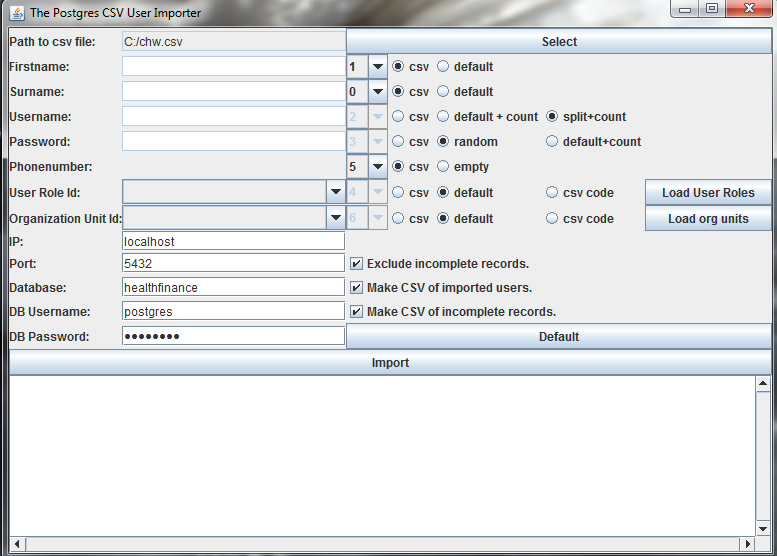
\includegraphics[width=\textwidth]{case/img/userImporterScreenShot}
\caption{Screen Shot of the User Importer}
\label{fig:screenUser}
\end{figure}

With setting up the mobile instance we also had to create the user accounts. 
The usual way of registering users in the \gls{dhis2} system is for an already registered user to navigate to the create user frame and input the information field by field. Firstname, surname, username, phone number, password and organization unit. With $\approx 45000$ users spread throughout all of Rwanda, this would clearly be a time consuming task. Fortunately we had a list of most of the \gls{chw}'s currently working in Rwanda. This list included all the required fields except username and password. We therefore chose to develop a small java application that could create the user accounts in the database. This application takes a .csv file as input were each row represents a \gls{chw}. The application generates a username based on their names and a random password for each \gls{chw}. After running the application, each \gls{chw} has a user account. There are some issues with doing it this way, like not involving the users in the process of registration. This might lead to users being registered and even don't know that the system exists and further leading to the system not being accepted. After the user is registered, the system are then able to recevie \gls{sms} reports from those users. 

\subsection{Re-Supply Algorithm}
The main purpose of the \gls{clmis} is of course to facilitate the process of delivering supplies and drugs to the individual \gls{chw}. Stock outs in this case is especially critical! Making sure that supplies are given at the right place at the right time requires a information system. In this case we want to have the information system estimate how much each village needs based on their consumption on a monthly basis. 

\begin{equation}
stk_{n} = stk_{n-1} + rcd_{n} - disp_{n}
\label{eq:basicEq}
\end{equation}

In equation \ref{eq:basicEq} we have the basic formula. How much a village have of an item at the end of month 'n' is what they had from last month, plus what they have received during month 
'n', minus what they have dispensed the same month. 

By reporting $stk_{n}$ each month we are able to choose between either reporting the quantity of received or dispensed. By reporting what is received, when received, it is easier to track the items. 

\begin{eqnarray}
reorder_{n} & = & (amc_{n} \cdot 2) - stk_{n} \\
amc_{n} & = & \frac{disp_{n-2} + disp_{n-1} + disp_{n}}{3} \\
disp_{n} & = & stk_{n-1} + rcd_{n} - stk_{n} \\
disp_{n-1} & = & stk_{n-2} + rcd_{n-1} - stk_{n-1} \\
disp_{n-2} & = & stk_{n-3} + rcd_{n-2} - stk_{n-2}
\label{eq:reorder}
\end{eqnarray}

Using this formula we are able to calculate both how much should be reordered and the average monthly consumption.


\begin{description}
\item[$\mathbf{reorder_{n}}$]
This variable represents the quantity of how much is needed at the next re-supply of one village. $n$ in this case represents the last month. If in May, it represents reorder quantity for the end of month of April.
\item[$\mathbf{amc_{n}}$]
Represents the average monthly consumption based on the last 3 months in one village. I in May, that would be the average monthly consumption based on February, March and April.
\item[$\mathbf{disp_{n}}$]
This variable is calculated based on the the values reported and is the number of items distributed by one village during one month.
\item[$\mathbf{stk_{n}}$]
The quantity in stock at the end of the month of one village. Usually reported within 1--5 days into the next month it represents. Stock in April is usually reported between 1st and 5th of May.
\item[$\mathbf{rcd_{n}}$]
This variable is the sum of items received in one village during the month it represents. If a \gls{chw} receives 10 condoms 2nd of April, it should be reported the same day. If a village receives another 10 condoms the 13th of April, that should also be reported the same day it is received. $rcd_{n}$ for April would then be the sum of those values, 20.

\begin{equation}
rcd_{n} = \sum_{k = 1}^{j} rcd_{n,k}
\label{eq:received}
\end{equation}.

\end{description}



A more mathematical description in equation \ref{eq:received}, where j represents the number of days in the month.

\subsubsection{The Essential Predictore}

\begin{figure}
\centering
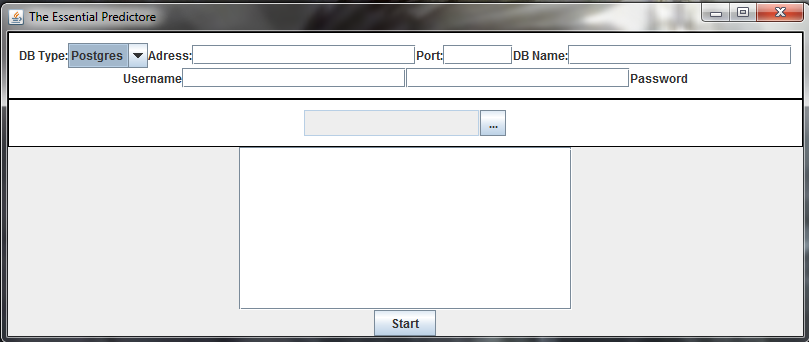
\includegraphics[width=\textwidth]{case/img/essentialPredictoreScreenShot}
\caption{Screen Shot of the Essential Predictore}
\label{fig:essPred}
\end{figure}

Based on the reorder algorithm we decided to make an application that would automatically calculate both $amc_{n}$, $reorder_{n}$ and make them available in \gls{dhis2}. This application was partly programmed in POSTGRESQL, then wrapped in JAVA. 
As seen in figure \ref{fig:essPred}, the applications takes as input the database information and a date. 
The application then calculates the values needed to update the tables in the \gls{dhis2} database. 
\gls{dhis2} has with the release after 2.15 made it possible to integrate \gls{dhis2} specific applications. 
If there is going to be a next version of the application it's decided that this will be an integrated application rather than a stand-alone JAVA application. 

\section{Demo 3}


\section{Case Summary}


\section{East Africa}

\section{DHIS2 Academy}
%
%\section{Notes}
%Based on the four objectives we made four use cases that was supposed to represent each one. Objective \#1 would be represented with use case \ref{tab:notifications}, objective \#2 with \ref{tab:reminders}, \#3 with \ref{tab:feedback} and \#4 with \ref{tab:smsreport}. These use cases worked as guidelines for our further work. They were not updated later on, because of the continuous updated requirements from \gls{chd} and other co-workers. That is one of the key characterizations of this project. The requirements kept on updating as more and more people got involved in the process. The more progress we made the less progress we made. As the project was coming more and more realized, more interest were made to the project, and more requirements were added. There were a kind of common understanding in the team. Once you got the picture, you didn't need to operate on a model anymore. Everyone kinda knew what needed to be done. The result of the diagnosis were essentially a clarification of what we were supposed to do and who are involved. The clients are \gls{chd}. A meeting took place and a list of contact information was exchanged. The users of the system are \gls{chw}'s, Cell \gls{chw} Supervisors, \gls{hc} \gls{chw} Supervisors and District Pharmacists. The basic idea is that the \gls{chd} would like to have \gls{hmis} make a system that enables \gls{chw}'s to report using \gls{sms} and based on this have automatic generated orders sent to the \gls{hc}'s and District Pharmacists.
%
%
%Our planning phase became somewhat glued together with the intervention. And continually altered. New problems were made visible by the interventions we made, and took us back to the planning phase. Making it very difficult to follow the action research model. In a perfect world, it is possible to plan everything to the point, but in our case new knowledge about the system was discovered along with our interventions and in turn, our plans had to be changed. 
%
%
%
%As seen in figure \ref{fig:chworder}, some overall plan were already in place. The result should be that the \gls{chw}'s should report what they receive whenever they receive any items. This will be registered in the database at the \gls{ndc}. 
%This would be straight from a village level to the national level. At the \gls{ndc} there will be a server running \gls{dhis2}, ready to receive data from MTN, the biggest mobile company in Rwanda. The \gls{sms} actually has to go through a \gls{smsc}, before being forwarded to the server at the \gls{ndc}. 
%The \gls{dhis2}-instance, from now called "the mobile instnce", will run all the necessary calculations and generate all the results. 
%So one of the tasks to be done was to set-up the mobile instance. 
%We knew that this would take some time, so in the mean time we sat up a test environment so that we could test our solutions. 
%
%
%\subsection{Intervention}
%
%\subsubsection{Setting up the Test Environment}
%Our initial idea was to set up a \gls{dhis2} instance for testing purposes. This made it possible for us to check if our objectives was in some way already met with the functionality of \gls{dhis2}. We knew that \gls{dhis2} already supported \gls{sms} reporting, but it had never been tested. This was essentially what we did. Configured \gls{dhis2} to support our case. Turned out that objective \#3 and \#4 was already met with just configuring \gls{dhis2}. One thing that we did not think about that became a problem later was the translation of the feedback messages. \gls{chw}'s do not generally speak English, but the local language kinyarwanda. Fortunately, the translation of the messages was possible in the next version of \gls{dhis2}, so the objective was still met. 
%
%We sat up the \gls{dhis2} instance at the \gls{ndc}. This is server that the \gls{chw}'s will send their reports to. This process was very straight forward. The problem with having our instance running at a different location is that we have less control of our system. Now we have to go through another team to make certain changes to the system. Actually just slows down the whole process. Setting up the mobile instance made our plans more real and allowed us to show our work in real life. 
%
%
%The user importer was made in order to import user from a csv file. \gls{dhis2} did not support automatically generating usernames and passwords for bulk users. Therefore we needed a program to do this for us. The down side of this approach is that all the users of the system are not included in the process of creating user accounts. This by passes the \gls{hisp} philosophy of including local users in the system. Users may therefore have user accounts they are not aware of. Making the the users feel less ownership of the system. Despite of this we decided to take this approach.The amount of resources spent on manually register all the users would be to vast. 	
%
%
%The user importer creates user accounts based on firstname, surname, village and phonenumber. After the user accounts are created they are able to send in \gls{sms}-reports based on the village they work from. 
%
%
%In order to generate the threshold values to send reminders from we chose to make a small application to run the algorithm. The application updates the database directly. The funny thing is that this was the only way we knew how to get our result, despite the support we had. The developer team from Oslo has offer the competence we needed, but due to the time frame we decided that we needed to build this application with SQL and JAVA. The application was kind of split in two. One of the team members at \gls{hmis} had a strong familiarity with databases and I had some JAVA experience. The core of the application was made in SQL, then it was wrapped inside a JAVA-\gls{gui}.
%
%
%The collaboration in this application is something worth taking note of. Neither one of the team member knew exactly what the other was doing. The application was in fact copy-pasted together after making the the \gls{gui} and SQL-functionality separately. The application realizes the re-supply algorithm in a JAVA application and works with \gls{dhis2}. So all the tools from \gls{dhis2} could be taken advantage of. 
